
\section{Background and Related Work}
\label{sec:backgr-relat-work}


\subsection{The MiGen system}
\label{sec:migen-system}

The MiGen project (http://www.migen.org) has designed and developed an
intelligent, exploratory environment to support 11 to 14-year-old
students in their learning of algebraic generalisation. Using a
mathematical microworld called the {\em eXpresser}, students construct
two-dimensional tiled patterns and derive general rules for the number
of tiles required to paint the pattern. 

Using the eXpresser, students are asked to construct
two-dimensional tiled patterns, which may be painted in different
colours, and to derive general rules for the number of tiles of each
colour required to paint each pattern and their model
overall. Students are prompted to create `building-blocks' to
construct their patterns, depending on their perceptions of the
pattern’s structure. Each building block is made up of a group of
tiles, and can be repeated horizontally, vertically or diagonally to
contribute to the construction of the pattern. For example, Figure 1
shows an example model that students may be asked to construct. They
may do so by creating building-blocks to
generate the centres of the flowers, the petals, and the stalks, and
will be nudged
towards deriving rules for the number of red tiles and the number of
green tiles required to paint the model, given the number of yellow
tiles.

\begin{figure}[htbp]
  \centering
  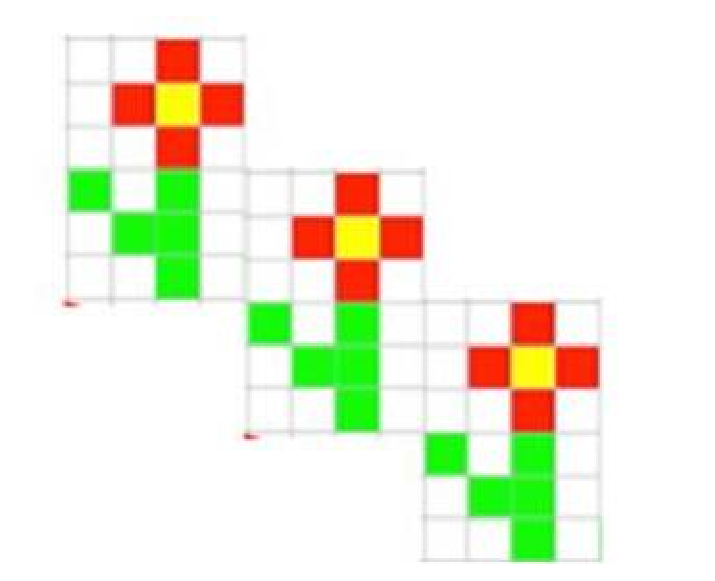
\includegraphics[width=6cm]{gfx/example.eps}
  \caption{An example model that students may be asked to construct in
    eXpresser} 
  \label{fig:example}
\end{figure}


Students are prompted to check that their models and rules are {\em
  general}, which they can accomplish by making appropriate use of
variables. For example, constructing the model in Figure 1 requires
one variable – for the number of yellow tiles. If the model has been
constructed generally by the student, changing the number of yellow
tiles will lead to it being updated correctly as a whole and also
still being correctly and fully coloured. The eXpresser has an
`animation' facility which allows students to explore the generality
of their models and rules. This facility automatically applies
different random values to the variables used by the student and
displays the resulting instances of the model in a separate pane of
their display screen.  

Tasks are designed to contextualise students' interaction with the
eXpresser and include a set of goals that students need to achieve,
e.g. `construct your model', `make sure it is correctly coloured',
`check that it animates without messing up', and `check that your
animated model is always correctly coloured'. The task goals are
presented to the student within an Activity Document, in which
students can tick off goals they believe they have completed, answer
questions relating to the task, reflect on their construction approach
etc. We refer the reader to [*MiGenJCAL] for details of 
further details of the eXpresser, its `epistemic
affordances' and how it can enhance
 students’ understanding of algebraic generalisation and to~\cite{CompAndEdPaper} for further details
of the system architecture, the Activity and Task design, and Activity Documents.  

Exploratory Learning Environments such as MiGen’s eXpresser
have the potential to support students' exploration while at the same
time fostering progressive building of knowledge. However, the
exploratory nature of the tasks undertaken with eXpresser requires
that personalised feedback is provided to students as they construct
their solutions, and not just at the end of the task. This feedback
includes prompts to help students engage with a task, improve their
solutions, reflect upon their interactions and guide them towards
successful completion of the task, and generalise their solutions
[*CompAndEndPaper, *relevantPapersOnIntSupport]. 

The feedback is generated by another
component of the MiGen system, the {\bf eGeneraliser}, based on an
analysis of students’ actions in the eXpresser. %
% and in MiGen we provide personalised feedback to students as they are
% undertaking their constructions, in the form of a series of prompts
% and nudges that help students reflect upon their interactions and
% guide them towards successful completion of the task. 
%
The aim of the
feedback is to balance students' freedom to explore while at the same
time providing sufficient support to ensure that learning is
achieved. We refer the reader to~\cite{relevantPapersOnIntSupport} for
details of the design of the eGeneraliser and of the feedback it
provides to students, and the way that this feedback is generated by
the system.  

\subsection{The problem}
\label{sec:problem}

Feedback generated by the eGeneraliser cannot cover all needs for help
of the students~\cite{ISmetrics}. In particular, there are three types
of support that are not covered by the eGeneraliser: very specific
conceptual difficulties, engagement nudges to prevent students from
getting distracted, and group support to help the classroom as a
group.\ednote{hostage to fortune}

Regarding the first type, the eGeneraliser can support students' work
at to a certain degree, but its ``intelligence'' is limited. There are
situations in which the feedback provided by the system is not
relevant to what the students are doing, or does not really help them
advance in the current task. There are also cases in which the
ambiguity of the students' actions requires a dialog with the student
to understand what they want to do and what kind of help they
need. When one of these situations arises, the teacher can come and
help the student. 

The second type of support is very simple but very necessary. The
target group age for the MiGen system is 11--14-year-old children. At
this age, is easy for learner to become distracted, even more so when
they are interacting with a computer connected to the
internet. Teachers need to remind students constantly to remain
on-task and avoid distractions. The MiGen system is only one
application in the student's computer, so it can detect distractions
(e.g. by detecting inactivity on eXpresser) but cannot do anything
about it. 

Finally, teachers want to support the whole class in two ways:
explaining common misconceptions to the whole class, if the need
arises, and steering their learning as a group to prevent ``fast''
students to become bored and ``slow'' students to become
frustrated. The eGeneraliser is a system that monitors only
individual interactions, not the whole group. 

These three types of support are necessary for a productive lesson
using a microworld like eXpresser, yet they can become very
challenging for a teacher without any additional support. Depending on
the classroom configuration, teacher cannot see all the students'
screens. Even if they do, the constant demands for their attention
makes it very difficult to monitor what thirty students are doing at
the same time. There is a clear need for computer-based support to
make teacher aware of what is happening so that they can act
accordingly. 

\subsection{Our approach}
\label{sec:our-approach}
 
As students are undertaking their tasks within the eXpresser, a series
of {\em indicators} are automatically detected by the eXpresser or
inferred by the eGeneraliser and are submitted by them to the MiGen
Server for storage in the MiGen database\footnote{The MiGen software
  comprises the eXpresser running on each student’s computer, the TA
  tools running on the teacher’s computer, and the MiGen Server and
  database running on a third computer. The MiGen database stores all
  the information produced and required by the eXpresser and the TA
  tools (see [CompAndEdPaper,IEEETLTPaper] for details).}.   
The set of indicators that are meaningful and useful for teachers in
their role in the classroom was identified through an iterative
process, undertaken collaboratively with our group of teacher
collaborators on the MiGen project (see Section~\ref{sec:methodology}).  

There are two categories of indicators: Task Independent (TI)
indicators refer to aspects of the student’s interactions that are
related to the eXpresser itself and do not depend on the specific task
the student is working on. TI indicators generally refer to a single
action undertaken by the student, such as ‘placed a tile on the
canvas’, ‘created a building-block’, ‘created a pattern’. In contrast,
the detection of Task Dependent (TD) indicators requires access to
knowledge about the task that the student is working on, it may relate
to combinations of actions by the student, and it requires intelligent
reasoning by the system. This reasoning is undertaken by the
eGeneraliser component, using a mixture of case-based and rule-based
techniques. Examples of TD indicators are `student has made a
plausible building block for this task’, ‘student has coloured their
pattern generally’ and `student has achieved a task goal'. Detailed
discussions of the MiGen's TI and TD indicators and how the latter are
inferred by the eGeneraliser may be found in~\cite{IEEETLTPaper}.
 
The {\bf TA Tools}
% , which are described in more detail in
% Section~\ref{sec:teach-assist-tools},
receive real-time information from the MiGen server relating to
occurrences of TI and TD indicators for each student, and each TA tool
presents a selection of this information in a visual fashion to the
teacher. The TA tools include the Student Tracking (ST) tool, the
Classroom Dynamics (CD) tool and the Goal Achievements (GA) tool. The
ST tool provides real-time visualisation of the occurrence of all TI
and TD indicators for each student as they are interacting with
eXpresser. 
% , showing these in one column of the display for each
% student, with time increasing downwards, and new information being
% added at the bottom of the display (see Figure\ref{eee}). Indicators
% are coloured Green if the occurrence of such an indicator indicates
% that the actions of the student are consistent with what would be
% expected by the system from constructive interaction, Red if the
% occurrence of such an indicator is regarded by the system as an
% obstruction to constructive interaction, Yellow if the occurrence of
% such an indicator indicates an aspect of the student’s interaction
% that may be positive or negative depending on the context, and Blue
% for indicators that represent feedback generated by the system for the
% student. Further details relating to Figure 2 and the ST tool are
% given in Section~\ref{sec:4.1}.
The CD tool represents the current status of each student in the
classroom. 
% visually as a circle whose colour
% is updated to reflect the current status of the student, which is one
% of: active and working constructively on the task (Green), inactive
% (Amber), and waiting for help from the teacher (Red) (see Figure 3). A
% small subset of the total TI/TD indicators are required to update this
% information, namely the indicators relating to students’
% activity/inactivity and students’ usage of the eXpresser’s help
% facility. If the teacher clicks on one of the circles in the CD
% display, that student’s current model and rule, as currently being
% worked on by the student in the eXpresser, is displayed to the teacher
% (see Figure\ref{fff}).
% 
The GA tool tracks progress in the current task's goals. 
% just one of the indicators - `student has achieved
% a task goal' - and shows visually, in the form of one row per student,
% the achievement of each task goal by each student (see Figure
% 5). Tasks shown as Green are currently achieved, those shown as White
% are currently not achieved, and those shown as Amber were achieved at
% some point during the student’s construction but are not being
% achieved by the current model.
Section~\ref{sec:methodology} explains the methodology we followed to
design these three tools to assist teachers in the classroom, and
Section~\ref{sec:teach-assist-tools} described the final result in
more detail. 

% REUSE SOMEWHERE
% The teacher can also select to see a summary of the goal achievement
% information within the CD tool by switching on a feature that displays
% within the student’s circle the number of goals achieved so far as a
% fraction of the total number of goals e.g. if the student has achieved
% 2 of a total of 4 task goals, this would show as “2/4” within the
% student’s circle. That feature has been enabled in the display shown
% in Figure\ref{4r4r}. 

\subsection{Related Work}
\label{sec:related}

In terms of related work, the work closest to MiGen’s TA tools is that
of [20] which uses Web log data generated by course management systems
(WebCT in their case) to help instructors be aware of students’
activities in distance learning classes; [21] which presents tools for
helping teachers understand students’ behaviour in adaptive tutorials
through post-analysis of the system’s data logs; [22] which presents
tools for teachers to visualise students’ progress through
simulation-based practical work sessions, and [23] which provides
awareness information to teachers so as to support their role as
moderators of multiple e-discussions.  

[*** SERGIO, these references are from the IEEE TLT paper; I guess we
need a, slimmed down, discussion of this work here; plus additional
relevant references ***] 
 
To our knowledge, MiGen’s TA tools represent the first work that is
targeted at notifying teachers of students’ progress during
constructionist learning activities in the classroom, notifying the
teacher of students’ attainment of key indicators, and aiming to
inform the teacher’s own interventions in the class. This novelty of
our TA tools has presented a number of methodological challenges,
which we discuss in Section 3.  

Discussion here also of other related work on: 
\begin{itemize}
\item  interaction analysis
\item  work on CSCL (even if we are not targetting collaboration here)
  to support teachers 
\item  work on teachers’ tools for moderating online discussions and
  argumentation 
\item  other tools for learning
\item Israel gutierrez's work on Interaction Analysis
\item Argonaut's teacher tools (Astrid Wichman, Ulrich Hoppe)
\end{itemize}


%%% Local Variables:
%%% mode: latex
%%% TeX-master: "main"
%%% End:
